
\documentclass{beamer}
\usecolortheme{dove}
\setbeamertemplate{navigation symbols}{}
\usepackage{amsmath,amssymb,amsfonts,amsthm, multicol, subfigure, color}
\usepackage{bm}
\usepackage{graphicx}
\usepackage{tabularx}
\usepackage{booktabs}
\usepackage{hyperref}
\usepackage{pdfpages}
\usepackage{xcolor}
\definecolor{seagreen}{RGB}{46, 139, 87}
\def\independenT#1#2{\mathrel{\rlap{$#1#2$}\mkern2mu{#1#2}}}
\newcommand\indep{\protect\mathpalette{\protect\independenT}{\perp}}
\def\log{\text{log}}
\newcommand\logit{\text{logit}}
\newcommand\iid{\stackrel{\text{iid}}{\sim}}
\newcommand\E{\text{E}}
\newcommand\V{\text{V}}
\renewcommand\P{\text{P}}
\newcommand{\Cov}{\text{Cov}}
\newcommand{\Cor}{\text{Cor}}
\newcommand\doop{\text{do}}
\usepackage{stackrel}
\usepackage{tikz}
\usetikzlibrary{arrows,shapes.arrows,positioning,shapes,patterns,calc}
\newcommand\slideref[1]{\vskip .1cm \tiny \textcolor{gray}{{#1}}}
\newcommand\red[1]{\color{red}#1}
\newcommand\blue[1]{\color{blue}#1}
\newcommand\gray[1]{\color{gray}#1}
\newcommand\seagreen[1]{\color{seagreen}#1}
\newcommand\purple[1]{\color{purple}#1}
\newcommand\orange[1]{\color{orange}#1}
\newcommand\black[1]{\color{black}#1}
\newcommand\white[1]{\color{white}#1}
\newcommand\teal[1]{\color{teal}#1}
\newcommand\magenta[1]{\color{magenta}#1}
\newcommand\Fuchsia[1]{\color{Fuchsia}#1}
\newcommand\BlueGreen[1]{\color{BlueGreen}#1}
\newcommand\bblue[1]{\textcolor{blue}{\textbf{#1}}}
\newcommand\bred[1]{\textcolor{red}{\textbf{#1}}}
\newcommand\bgray[1]{\textcolor{gray}{\textbf{#1}}}
\newcommand\bgreen[1]{\textcolor{seagreen}{\textbf{#1}}}
\newcommand\bref[2]{\href{#1}{\color{blue}{#2}}}
\colorlet{lightgray}{gray!40}
\pgfdeclarelayer{bg}    % declare background layer for tikz
\pgfsetlayers{bg,main} % order layers for tikz
\newcommand\mycite[1]{\begin{scriptsize}\textcolor{darkgray}{(#1)}\end{scriptsize}}
\newcommand{\tcframe}{\frame{
%\small{
\only<1|handout:0>{\tableofcontents}
\only<2|handout:1>{\tableofcontents[currentsubsection]}}
%}
}

\usepackage[round]{natbib}
\bibliographystyle{humannat-mod}
\setbeamertemplate{enumerate items}[default]
\usepackage{mathtools}

\newcommand{\goalsframe}{\begin{frame}{Learning goals for today}
\begin{itemize}
    \item fork structures
    \item collider structures
    \item causal reasoning and statistical independence
\end{itemize} \vskip .2in
\end{frame}}

\title{Causal Inference 2: Directed Acyclic Graphs}
\author{Ian Lundberg\footnote{Assistant Professor, Information Science, Cornell, \href{mailto:ilundberg@cornell.edu}{ilundberg@cornell.edu}} \& Kristin Liao\footnote{PhD Student, Sociology, UCLA, \href{mailto:ktliao@g.ucla.edu}{ktliao@g.ucla.edu}}}
\date{SICSS UCLA\\25 June 2024}

\begin{document}

\maketitle

\goalsframe

\begin{frame}{A hypothetical experiment in two population subgroups}

\begin{tikzpicture}[x = \textwidth, y = .7\textheight]
\node at (0,0) {};
\node at (1,1) {};
\pause
\node[anchor = north west, align = left] (l1) at (0,1) {People who like exercise};
\node[anchor = north west, align = left] (l0) at (.5,1) {People who don't like exercise};
\draw[thick] (l1.south west) -- (l1.south east);
\draw[thick] (l0.south west) -- (l0.south east);
\pause
\node[anchor = north west, align = left] at (0,.8) {\textbf{Treatment}\\75\% assigned an exercise\\coach for 1 month};
\node[anchor = north west, align = left] at (.5,.8) {\textbf{Treatment}\\25\% assigned an exercise\\coach for 1 month};
\pause
\node[anchor = north west, align = center] at (0,.5) {\textbf{Outcome}: How many pull-ups can they do?};
\pause
\node[anchor = north west, align = left] at (0,.3) {\textbf{Question for you:}\\Give 2 reasons why those assigned a coach can do more pull-ups};
\end{tikzpicture}

\end{frame}

\begin{frame}{A hypothetical experiment in two population subgroups}
\begin{center}
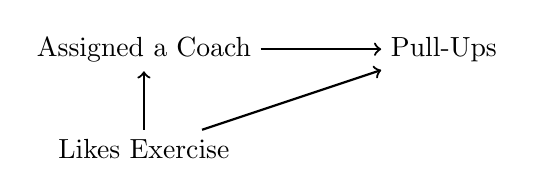
\begin{tikzpicture}[x = 1.5in, y = .5in]
\node (a) at (1,0) {Assigned a Coach};
\node (y) at (2,0) {Pull-Ups};
\draw[->, thick] (a) -- (y);
\node (l) at (1,-1) {Likes Exercise};
\draw[->, thick] (l) -- (a);
\draw[->, thick] (l) -- (y);
\end{tikzpicture}
\end{center} \pause
\textbf{Nodes} are random variables. \textbf{Edges} ($\rightarrow$) are causal relations \vskip .1in \pause
The graph links causal assumptions to statistical dependence
\vskip .2in \pause
In this graph, (Assigned a Coach) and (Pull-Ups) are statistically dependent because of two open paths:
\begin{itemize} \pause
\item (Assigned a Coach) $\rightarrow$ (Pull-Ups)
\begin{itemize}
\item a causal path: all arrows go one direction
\end{itemize} \pause
\item (Assigned a Coach) $\leftarrow$ (Likes Exercise) $\rightarrow$ (Pull-Ups)
\begin{itemize}
\item a backdoor path containing a fork
\end{itemize}
\end{itemize}
\end{frame}

\begin{frame}{A hypothetical experiment in two population subgroups}
\begin{center}
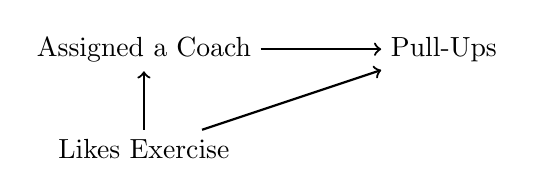
\begin{tikzpicture}[x = 1.5in, y = .5in]
\node (a) at (1,0) {Assigned a Coach};
\node (y) at (2,0) {Pull-Ups};
\draw[->, thick] (a) -- (y);
\node (l) at (1,-1) {Likes Exercise};
\draw[->, thick] (l) -- (a);
\draw[->, thick] (l) -- (y);
\end{tikzpicture}
\end{center}
How to study the causal effect (Assigned a Coach) $\rightarrow$ (Pull-Ups)? \pause
\begin{itemize}
\item split into two subgroups: likes exercise and don't \pause
\item we have a simple randomized experiment within each subgroup \pause
\item estimate within each subgroup \pause
\item pool the two estimates for an average causal effect estimate \pause
\end{itemize}
Terminology: Identify by \textbf{conditioning} on (Likes Exercise)
\end{frame}

\begin{frame}{Colliders: The sprinkler example}{Example from Pearl, J. (1988). Probabilistic Reasoning in Intelligent Systems: Networks of Plausible Inference.} \pause
\begin{itemize}
\item I set my sprinklers to turn on at random times \pause
\item It rains at random times \pause
\item (Sprinklers) or (Rain) can make the grass wet
\end{itemize} \pause
\begin{center}

\begin{tikzpicture}[x = 1.5in, y = .2in]
\node (s) at (1,1) {Sprinklers On};
\node (r) at (1,-1) {Raining};
\node (g) at (2,0) {Grass Wet};
\draw[->, thick] (s) -- (g);
\draw[->, thick] (r) -- (g);
\end{tikzpicture}
\end{center} \pause
Questions for you:
\begin{itemize}
\item Are (Sprinklers On) and (Raining) statistically dependent?
\item Are (Sprinklers On) and (Raining) statistically dependent\\once I restrict to times when the (Grass Wet = \texttt{TRUE})?
\end{itemize}

\end{frame}

\begin{frame}{Colliders: The sprinkler example}{Example from Pearl, J. (1988). Probabilistic Reasoning in Intelligent Systems: Networks of Plausible Inference.}
\begin{center}

\begin{tikzpicture}[x = 1.5in, y = .2in]
\node (s) at (1,1) {Sprinklers On};
\node (r) at (1,-1) {Raining};
\node (g) at (2,0) {Grass Wet};
\draw[->, thick] (s) -- (g);
\draw[->, thick] (r) -- (g);
\end{tikzpicture}
\end{center} \pause
\begin{itemize}
\item (Grass Wet) is a \textbf{collider}\hfill (arrows collide $\rightarrow\leftarrow$) \pause
\item A collider blocks a path
\begin{itemize}
\item marginal independence of (Sprinklers On) and (Raining) \pause
\end{itemize}
\item Conditioning on a collider opens the path
\begin{itemize}
\item conditional dependence of (Sprinklers On) and (Raining)\\when restricting to times when (Grass Wet = \texttt{True})
\end{itemize}
\end{itemize}
\end{frame}

\begin{frame}{Using DAGs to identify causal effects: Game plan} \pause

\begin{enumerate}[<+->]
\item Draw a DAG
\begin{itemize}
\item Create nodes for treatment and outcome
\item Add other nodes
\begin{itemize}
\item anything causally related to any two nodes in the graph
\item also add the causal edges
\end{itemize}
\end{itemize}
\item List all paths between treatment and outcome
\item Choose a sufficient adjustment set:\\variables that jointly block all non-causal paths
\begin{itemize}
\item a path is blocked if it contains an adjusted non-collider
\item a path is blocked if it contains an unadjusted collider\\(and no descendant of that collider is adjusted)
\item otherwise unblocked
\end{itemize}
\end{enumerate}

\end{frame}

\begin{frame}{Practice}

\Large
To what extent does completing a 4-year college degree affect a person's future earnings?

\end{frame}

\begin{frame}[t]{Effect of a 4-year degree on future earnings} \vskip .2in
\textbf{1) Draw a DAG} \pause \vskip .1in
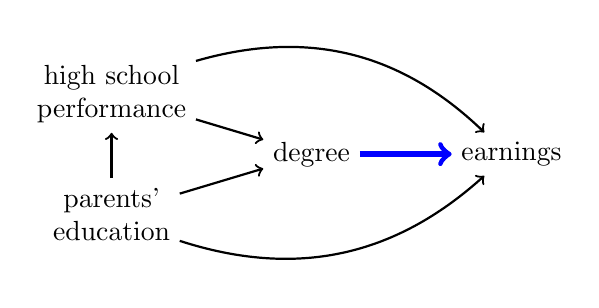
\begin{tikzpicture}[x = 1in, y = .3in]
\node (a) at (2,0) {degree};
\node (y) at (3,0) {earnings};
\pause
\draw[->, line width = 2pt, blue] (a) -- (y);
\pause
\node[align = center] (h) at (1,1) {high school\\performance};
\draw[->, thick] (h) -- (a);
\draw[->, thick] (h) to[bend left] (y);
\pause
\node[align = center] (p) at (1,-1) {parents'\\education};
\draw[->, thick] (p) -- (h);
\draw[->, thick] (p) -- (a);
\draw[->, thick] (p) to[bend right] (y);
\end{tikzpicture}
\end{frame}

\begin{frame}[t]{Effect of a 4-year degree on future earnings} \vskip .2in
\textbf{2) List all paths between the treatment and outcome} \vskip .1in
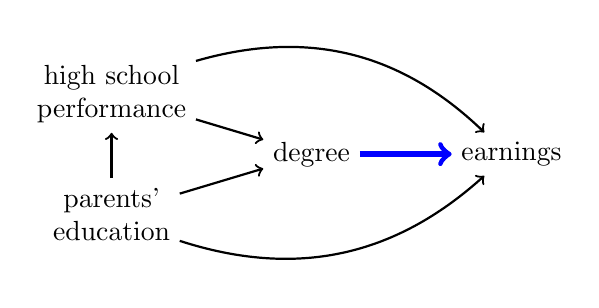
\begin{tikzpicture}[x = 1in, y = .3in]
\node (a) at (2,0) {degree};
\node (y) at (3,0) {earnings};
\draw[->, line width = 2pt, blue] (a) -- (y);
\node[align = center] (h) at (1,1) {high school\\performance};
\draw[->, thick] (h) -- (a);
\draw[->, thick] (h) to[bend left] (y);
\node[align = center] (p) at (1,-1) {parents'\\education};
\draw[->, thick] (p) -- (h);
\draw[->, thick] (p) -- (a);
\draw[->, thick] (p) to[bend right] (y);
\end{tikzpicture} \pause

Causal paths\vskip .03in
\begin{footnotesize}
(degree) $\rightarrow$ (earnings)
\end{footnotesize} \vskip .1in \pause
Backdoor paths\vskip .03in
\begin{footnotesize}
(degree) $\leftarrow$ (high school performance) $\rightarrow$ (earnings) \\
(degree) $\leftarrow$ (parents' education) $\rightarrow$ (earnings) \\
(degree) $\leftarrow$ (high school performance) $\leftarrow$ (parents' education) $\rightarrow$ (earnings)
\end{footnotesize}
\end{frame}

\begin{frame}[t]{Effect of a 4-year degree on future earnings} \vskip .2in
\textbf{3) Choose a sufficient adjustment set}\\\textbf{\{high school performance, parents' education\}}
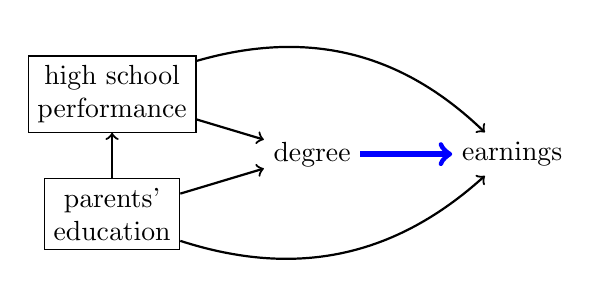
\begin{tikzpicture}[x = 1in, y = .3in]
\node (a) at (2,0) {degree};
\node (y) at (3,0) {earnings};
\draw[->, line width = 2pt, blue] (a) -- (y);
\node[align = center, draw] (h) at (1,1) {high school\\performance};
\draw[->, thick] (h) -- (a);
\draw[->, thick] (h) to[bend left] (y);
\node[align = center, draw] (p) at (1,-1) {parents'\\education};
\draw[->, thick] (p) -- (h);
\draw[->, thick] (p) -- (a);
\draw[->, thick] (p) to[bend right] (y);
\end{tikzpicture}

Causal paths\vskip .03in
\begin{footnotesize}
(degree) $\rightarrow$ (earnings)
\end{footnotesize} \vskip .1in
Backdoor paths\vskip .03in
\begin{footnotesize}
(degree) $\leftarrow$ \boxed{\text{high school performance}} $\rightarrow$ (earnings) \\
(degree) $\leftarrow$ \boxed{\text{parents' education}} $\rightarrow$ (earnings) \\
(degree) $\leftarrow$ \boxed{\text{high school performance}} $\leftarrow$ \boxed{\text{parents' education}} $\rightarrow$ (earnings)
\end{footnotesize}
\end{frame}

\begin{frame}{DAGs: A promising path}

\begin{itemize}
\item DAGs connect causal theories to statistical dependence
\item Statistical dependence arises through causal paths
\item Paths may contain two key structures
\begin{itemize}
\item forks: $A\leftarrow B \rightarrow C$\\($A$ and $C$ dependent if $B$ unadjusted)
\item colliders: $A \rightarrow B \leftarrow C$\\($A$ and $C$ dependent if $B$ adjusted)
\end{itemize}
\item Causal identification goal:\\choose a sufficient adjustment set so only the causal path of interest remains open
\item Experimental analog:\\Among units who are identical on the sufficient adjustment set, we have a simple randomized experiment
\end{itemize}

\end{frame}

\begin{frame}{DAGs: Words of warning} \pause

Inference is only valid to the degree that the DAG holds\pause
\begin{itemize}
\item Your claim:\\If this is the DAG,\\then adjusting for $\vec{X}$ identifies the effect
\end{itemize} \pause \vskip .2in
It is important to reason about when the DAG may not hold \pause
\begin{center}
\begin{tikzpicture}[x = 1in, y = .3in]
\node at (2,2.5) {};
\node (a) at (2,0) {degree};
\node (y) at (3,0) {earnings};
\draw[->, line width = 2pt, blue] (a) -- (y);
\node[align = center, draw] (h) at (1,1) {high school\\performance};
\draw[->, thick] (h) -- (a);
\draw[->, thick] (h) to[bend left] (y);
\node[align = center, draw] (p) at (1,-1) {parents'\\education};
\draw[->, thick] (p) -- (h);
\draw[->, thick] (p) -- (a);
\draw[->, thick] (p) to[bend right] (y);
\only<6>{
\node[font = \bf, red] (u) at (2.5,2) {Motivation};
\draw[->, red, line width = 2pt, dashed] (u) to[bend right] (a);
\draw[->, red, line width = 2pt, dashed] (u) to[bend left] (y);
}
\only<7>{
\node[font = \bf, red] (u) at (2.5,2) {Social Ties};
\draw[->, red, line width = 2pt, dashed] (u) to[bend right] (a);
\draw[->, red, line width = 2pt, dashed] (u) to[bend left] (y);
}
\only<8>{
\node[font = \bf, red] (u) at (2.5,2) {Cultural Capital};
\draw[->, red, line width = 2pt, dashed] (u) to[bend right] (a);
\draw[->, red, line width = 2pt, dashed] (u) to[bend left] (y);
}
\end{tikzpicture}
\end{center}
\end{frame}

\begin{frame}{Resources to learn more}

\begin{itemize}
\item Hernán, M.A., \& J.M. Robins. 2020.\\\bref{https://www.hsph.harvard.edu/miguel-hernan/causal-inference-book/}{Causal Inference: What If?}\\Boca Raton: Chapman \& Hall / CRC.
\item Pearl, J., \& Mackenzie, D. (2018).\\\bref{https://www.hachettebookgroup.com/titles/judea-pearl/the-book-of-why/9781541698963/?lens=basic-books}{The Book of Why: The New Science of Cause and Effect.}\\Basic Books.
\item Pearl, J., Glymour, M., \& Jewell, N. P. (2016).\\\bref{https://www.wiley.com/en-us/Causal+Inference+in+Statistics\%3A+A+Primer-p-9781119186847}{Causal Inference in Statistics: A Primer.}\\John Wiley \& Sons.
\item Pearl, J. (2000).\\\bref{https://www.cambridge.org/core/books/abs/causality/contents/E62B1C761BC88EF7A8FE13A25FDFBBCD}{Causality.}\\Cambridge University Press.
\end{itemize}

\end{frame}

\end{document}